\باب{سوالات}

\حصہء{میکس ویل مساوات}
%====================
\ابتدا{سوال}
رداس \عددی{\rho=\SI{12}{\centi\meter}} کے گول دائرے میں وقت کے ساتھ تبدیل ہوتا، یکساں مقناطیسی میدان \عددی{B(t)=0.15\sin 1000 t \, \si{\weber}} ہے جو دائرے میں محرک برقی دباو \عددی{e(t)} پیدا کرتا ہے۔گول دائرے کی مزاحمت \عددی{\SI{55}{\ohm}} ہے۔محرک برقی دباو،  گول دائرے میں برقی رو \عددی{i(t)} پیدا کرتی ہے۔برقی رو \عددی{i(t)} سے پیدا مقناطیسی بہاو کو نظر انداز کرتے ہوئے \عددی{e(t)} اور \عددی{i(t)} حاصل کریں۔صورت حال شکل \حوالہ{شکل_سوال_میکس_ویل_دائرہ_محرک_دباو} میں دکھائی گئی ہے جہاں صفحہ سے اوپر کی جانب باہر نکلتی مقناطیسی میدان کو چھوٹے دائروں میں بند نقطوں سے ظاہر کیا گیا ہے۔
\begin{figure}
\centering
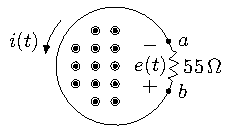
\includegraphics{figMaxwellRingEMF}
\caption{دائرے میں یکساں مقناطیسی بہاو، محرک برقی دباو پیدا کرتا ہے۔}
\label{شکل_سوال_میکس_ویل_دائرہ_محرک_دباو}
\end{figure}

جوابات:\عددی{-6.78 \cos 1000t \, \si{\volt}}، \عددی{-123\cos 1000t \, \si{\milli\ampere}}
\انتہا{سوال}
%======================
\ابتدا{سوال}
سطح \عددی{z=0} پر موصل تار کے مستطیل کے اطراف \عددی{x=\mp \SI{2}{\meter}}، \عددی{y=\mp\SI{1.5}{\meter}} پر ہیں۔وقت کے ساتھ تبدیل ہوتا مقناطیسی میدان \عددی{\kvec{B}=(0.25\ax-0.55\ay+0.1\az)\sin 1200 t \, \si{\tesla}} ہے۔مستطیل کی کل مزاحمت \عددی{R=\SI{4200}{\ohm}} ہے۔مثبت \عددی{z} محدد کی جانب سے دیکھتے ہوئے، گھڑی کی سمت میں برقی رو حاصل کریں۔برقی رو سے پیدا ثانوی مقناطیسی میدان کو نظر انداز کرتے ہوئے حل کریں۔

جواب:\عددی{343 \cos 1200 t \, \si{\milli\ampere}} 
\انتہا{سوال}
%=======================
\ابتدا{سوال}
مقناطیسی میدان \عددی{\kvec{B}=5\cos(1.2\times 10^{8} \pi t -\pi y)\az \, \si{\micro \tesla}} ہے۔مندرجہ ذیل فرضی یا غیر موصل دائروں پر \عددی{\aphi} سمت میں بڑھتا محرک برقی دباو حاصل کریں۔الف) \عددی{(0,0,0)} تا \عددی{(1,0,0)} تا \عددی{(1,1,0)} تا \عددی{(0,1,0)} تا \عددی{(0,0,0)}؛ ب) \عددی{(0,0,0)} تا \عددی{(2,0,0)} تا \عددی{(2,2,0)} تا \عددی{(0,2,0)} تا \عددی{(0,0,0)} 

جوابات:\عددی{600[\cos(1.2\times 10^{8} \pi t -\pi)-\cos (1.2 \times 10^{8} \pi t)] \, \si{\volt}}، \عددی{\SI{0}{\volt}}
\انتہا{سوال}
%=================
\ابتدا{سوال}
رداس \عددی{\rho=\SI{1}{\milli\meter}} اور \عددی{\rho=\SI{3}{\milli\meter}} کے ہم محوری تار
 میں \عددی{\kvec{H}=\tfrac{0.122}{\rho}\cos 5\times 10^{8} \pi t \cos 0.5 \pi z \aphi \, \si{\ampere\per\meter}} پایا جاتا ہے۔مستطیل \عددی{(0.001,0^{\circ},0)} تا \عددی{(0.003,0^{\circ},0)} تا \عددی{(0.003,0^{\circ},1.5)} تا \عددی{(0.001,0^{\circ},1.5)} تا \عددی{(0.001,0^{\circ},0)}   میں محرک برقی دباو حاصل کریں۔

جواب:\عددی{119\sin(5\times 10^{8}\pi t) \, \si{\volt}}
\انتہا{سوال}
%==================
\ابتدا{سوال}
لمحہ \عددی{t=0} پر موصل تار کے مستطیل کے اطراف \عددی{x=\SI{\mp 0.4}{\meter}} اور \عددی{y=\SI{\mp 0.6}{\meter}} پر ہیں۔یہ مستطیل \عددی{6 \ay \, \si{\meter\per\second}} کی سمتی رفتار سے حرکت کر رہی ہے۔غیر یکساں مقناطیسی میدان \عددی{\kvec{B}=3x^2y \az \, \si{\tesla}} ہے۔مستطیل کی مزاحمت \عددی{R=\SI{100}{\ohm}} ہے۔مستطیل میں طاقت کی اخراج حاصل کریں۔ساکن سلاخوں میں کتنی محرک برقی دباو پیدا ہوتی ہے۔  

جواب:\عددی{P=\SI{2.12}{\milli\watt}}، \عددی{\SI{0}{\volt}}
\انتہا{سوال}
%==================
\ابتدا{سوال}
شکل \حوالہ{شکل_میکس_ویل_سوال_محرک_سلاخ_ترچھی_ریل} میں دو ساکن موصل سلاخ \عددی{x} محدد کے ساتھ \عددی{\mp 10^{\circ}} کا زاویہ بناتے ہیں۔صفحہ کے بالائی سطح سے نکلتی مقناطیسی میدان \عددی{B=0.5\az \si{\tesla}} ہے۔ محرک سلاخ کی رفتار \عددی{v=\SI{8}{\meter\per\second}} ہے۔ ساکن سلاخوں کے بائیں سروں کے مابین آلہ پیما برقی دباو یوں نسب کیا گیا ہے کہ یہ \عددی{v_{ab}} ناپے۔ الف) محرک سلاخ کے مقام کو \عددی{t=0} پر \عددی{x=0} لیتے ہوئے آلہ پیمائش پر حاصل برقی دباو کی مساوات حاصل کریں۔ ب) محرک سلاخ کا مقام \عددی{x=50t^2 \, \si{\meter\per\second}} ہونے کی صورت میں جواب حاصل کریں۔
\begin{figure}
\centering
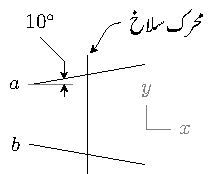
\includegraphics{figMaxwellSlidingConductorAngledRails}
\caption{محرک سلاخ پر مقناطیسی میدان محرک دباو پیدا کرتا ہے۔}
\label{شکل_میکس_ویل_سوال_محرک_سلاخ_ترچھی_ریل}
\end{figure}

جوابات:\عددی{}، \عددی{} 
\انتہا{سوال}
%==================
